\section{DESIGN DE INTERFACE}

Quem procura um animal perdido costuma abrir o aplicativo com pressa, sob tensão e, muitas vezes, na rua, com uma só mão livre. Nessas condições, uma tela confusa ou um campo ambíguo pode atrasar a publicação do alerta ou levar a informações incompletas. Por isso, o projeto de interface do WeFIND buscou reduzir a carga cognitiva do usuário, como recomendam Rogers, Sharp e Preece (2023), com telas diretas, organizadas e de navegação previsível.

No WeFIND, a construção das telas foi orientada por critérios de usabilidade, com destaque para as dez heurísticas de Nielsen (1994) adaptadas ao contexto dos smartphones e para as orientações da norma ABNT NBR ISO 9241-11 (ABNT, 2021). A norma define usabilidade a partir de eficácia, eficiência e satisfação. Esses princípios orientaram a organização dos fluxos de navegação, cadastro e registro de avistamentos; a experiência dos usuários foi verificada na avaliação descrita no Capítulo~8.

Outro cuidado central foi a acessibilidade digital, orientada pelas Diretrizes de Acessibilidade para Conteúdo Web (WCAG 2.2), no nível recomendado AA (W3C, 2023). No WeFIND, essas diretrizes serviram como referência para decisões de contraste, legibilidade e dimensões das áreas de toque, especialmente considerando o uso do smartphone em ambientes externos. A aderência a essas diretrizes foi examinada por inspeção das telas e pelo cálculo do contraste das cores principais; como mostra a Seção~7.3, algumas combinações ainda não atingem o mínimo do nível AA, de modo que o aplicativo não pode ser considerado plenamente conforme à WCAG 2.2.

Dessa maneira, o projeto visual buscou harmonizar clareza de informações, ergonomia e acolhimento. As subseções a seguir apresentam as escolhas tipográficas, a identidade visual, a paleta de cores e os principais fluxos de telas da plataforma WeFIND.


\subsection{Tipografia e Hierarquia Visual}

A tipografia contribui para a leitura e para a organização das informações nas telas do WeFIND. Em situações de busca, títulos, dados do animal e orientações precisam ser distinguidos com clareza. Por isso, a Roboto foi definida como referência tipográfica do projeto, com variações de peso e tamanho para estabelecer níveis de destaque, conforme apresentado na Figura~\ref{fig:tipografia}.

\begin{figure}[H]
    \centering
    \caption{Família tipográfica Roboto e hierarquia visual definidas para o WeFIND}
    \label{fig:tipografia}
    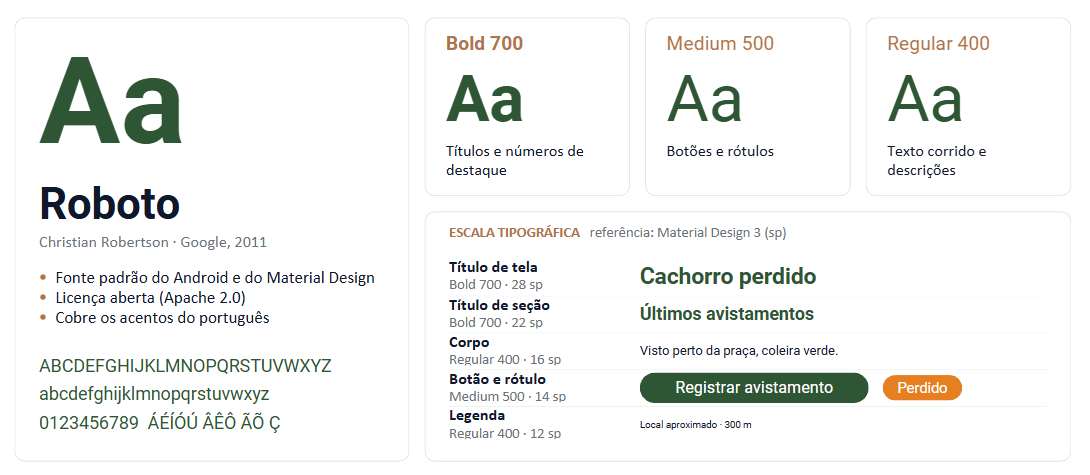
\includegraphics[width=\textwidth]{imagens/03_arquitetura_design/figura15_tipografia_roboto_v2.png}
    \fonte{Autoria própria (2026), com base em Google Fonts (2024) e Google (2026)}
\end{figure}

A Figura~\ref{fig:tipografia} apresenta a família Roboto, criada por Christian Robertson para o Google em 2011, fonte padrão do Android e do Material Design, distribuída sob licença aberta (Apache 2.0) e com suporte aos acentos do português. A figura reúne o alfabeto, os números e os caracteres acentuados, além dos pesos e tamanhos definidos como referência. A hierarquia prevê Roboto Bold (700) para títulos e números de destaque; Roboto Medium (500) para botões, rótulos e destaques de interface; e Roboto Regular (400) para textos corridos e descrições. A escala tipográfica toma como referência o Material Design 3 (Google, 2026) e utiliza a unidade sp (\textit{scale-independent pixels}), que acompanha o tamanho de fonte configurado pelo usuário no dispositivo: 28 sp para títulos de tela, 22 sp para títulos de seção, 16 sp para o corpo do texto, 14 sp para botões e rótulos e 12 sp para legendas. Os exemplos da figura, como ``Cachorro perdido'' e ``Registrar avistamento'', mostram a aplicação dessa escala em elementos reais da interface.


\subsection{Identidade Visual}

A identidade visual do WeFIND foi projetada para transmitir sentimentos de solidariedade comunitária, segurança, afeto e esperança. O próprio nome une o pronome inglês ``We'' (nós) ao verbo ``Find'' (encontrar), expressando a ideia de que a busca por um animal não é um esforço individual, mas uma tarefa compartilhada por toda a vizinhança.

A inclusão conjunta do cão e do gato no símbolo gráfico reflete a realidade do convívio familiar brasileiro. Embora muitas campanhas de proteção animal concentrem-se historicamente apenas em cães, a perda e o abandono de felinos também são frequentes e dolorosos no ambiente urbano. Ao reunir as duas espécies, a marca mostra desde o primeiro contato que a plataforma atende tutores de ambos com a mesma atenção.

Para a concepção do ícone oficial, utilizou-se o ChatGPT (OpenAI, 2026) como ferramenta de inteligência artificial generativa, integrado ao processo de design no Figma. A ferramenta auxiliou na exploração de composições visuais e na definição de um conceito moderno e equilibrado.

Os critérios solicitados incluíram estilo minimalista e plano, adequado para ícones em telas móveis de diversos tamanhos. Buscou-se a integração harmoniosa de silhuetas representativas do universo doméstico: o perfil amigável de um cão e de um gato, simbolizando as principais espécies acolhidas pelas famílias. No centro, posicionou-se o marcador de mapa, representando a busca baseada em localização, com as cores terracota e verde sobre fundo branco:

\begin{quote}
\small\textit{``Minimalist flat app icon for a lost and found pet mobile app, combining a friendly dog silhouette and a cat silhouette surrounding a central GPS location pin, solid colors forest green and terracotta, clean white background, modern vector logo design, no gradients, no photorealism.''}
\end{quote}

A partir do vetor gerado, realizou-se o refinamento manual no Figma, ajustando curvas, espessuras e simetria para garantir nitidez em telas menores. O logotipo final resultante desse processo é apresentado na Figura~\ref{fig:logotipo}.

\begin{figure}[H]
    \centering
    \caption{Logotipo Oficial e Ícone do Aplicativo WeFIND}
    \label{fig:logotipo}
    \includegraphics[width=0.42\textwidth]{imagens/03_arquitetura_design/figura13_logotipo_wefind.png}
    \fonte{Autoria própria (2026), com auxílio de ferramenta de inteligência artificial}
\end{figure}

O símbolo gráfico reúne a silhueta de um cão à esquerda e de um gato à direita, circundando o marcador clássico de localização geográfica ao centro. Essa composição sintetiza a missão do sistema de atender às principais espécies domésticas, enquanto o marcador central enfatiza o recurso de geolocalização em mapa. As cores aplicadas reforçam a proposta: o tom Terracota acolhe as silhuetas dos animais e o Verde Esperança colore o pino de localização.

A leitura do símbolo comunica com clareza o propósito da ferramenta. A forma circular vazada no centro do marcador geográfico atua como uma lente de foco, sugerindo a atenção comunitária voltada para avistar, localizar e reencontrar o animal desaparecido.

O símbolo foi também preparado para atender às exigências técnicas dos sistemas móveis contemporâneos, como os ícones adaptativos do Android, que utilizam máscaras de corte circulares e quadradas com áreas de segurança bem definidas. O ícone também conta com versão monocromática para a barra de notificações do celular, facilitando o reconhecimento imediato de alertas e mensagens.

Na interface do aplicativo, a marca é utilizada de maneira consistente na tela inicial de apresentação e nos cartazes digitais de busca. Essa padronização busca reforçar a identificação visual da plataforma e associá-la à proposta de apoio ao bem-estar animal.


\subsection{Paleta de Cores}

A definição cromática do WeFIND baseou-se nos princípios da psicologia das cores aplicados ao design digital (Heller, 2021), buscando transmitir serenidade e afeto sem prejudicar a visibilidade de avisos urgentes. A Figura~\ref{fig:paleta_cores} apresenta a paleta oficial do sistema, organizada em três grupos estruturados.

\begin{figure}[H]
    \centering
    \caption{Identidade Visual e Paleta Cromática Oficial do WeFIND}
    \label{fig:paleta_cores}
    \includegraphics[width=0.68\textwidth]{imagens/03_arquitetura_design/figura14_paleta_cores.jpeg}
    \par\vspace{0.15cm}
    {\footnotesize Figura~\thefigure.a) Cores da Plataforma \quad\textbar\quad Figura~\thefigure.b) Publicações \quad\textbar\quad Figura~\thefigure.c) Interface e Neutros\par}
    \fonte{Autoria própria (2026)}
\end{figure}

A organização das cores na Figura~\ref{fig:paleta_cores} estrutura-se em três blocos funcionais:

Na Figura~\ref{fig:paleta_cores}.a, apresentam-se as Cores da Plataforma. A Cor Primária em tom Verde (\#2E5634) evoca sentimentos de equilíbrio, esperança e solidez, sendo empregada como cor de fundo das barras superiores de navegação e em botões principais de ação. A Cor Secundária em tom Terracota (\#B1734A) remete ao cuidado, afeto e acolhimento animal, sendo utilizada em elementos secundários e detalhes de destaque.

Na Figura~\ref{fig:paleta_cores}.b, encontram-se as Cores Semânticas de Publicação, concebidas para permitir a triagem visual rápida do status de cada publicação: o tom Laranja Alerta (\#E67E22) sinaliza animais Perdidos; o Verde Sucesso (\#16A34A) identifica animais já Encontrados; o Magenta (\#BE185D) identifica os animais disponíveis para adoção; e o tom Amarelo Dourado (\#D4AC0D) destaca Avisos urgentes e novos relatos de avistamento comunitário.

Na Figura~\ref{fig:paleta_cores}.c, reúnem-se as Cores de Interface e Elementos Neutros: a tonalidade cinza suave de Fundo (\#F6F8F6) foi escolhida para favorecer o conforto visual; o tom branco puro de Superfície (\#FFFFFF) destaca cartões e campos interativos; e a tipografia principal em tom Azul Noturno Escuro (\#0F172A) foi selecionada para favorecer o contraste entre texto e fundo. A conformidade efetiva com os critérios aplicáveis da WCAG depende de verificação específica para cada combinação de cores e contexto de uso. Pelo cálculo da razão de contraste definida na WCAG 2.2, o texto branco sobre o verde primário (\#2E5634) atinge cerca de 8,4:1, acima do mínimo de 4,5:1 exigido para texto comum no nível AA; já o texto branco sobre o terracota (\#B1734A), o laranja (\#E67E22), o verde de sucesso (\#16A34A) e o amarelo (\#D4AC0D) fica abaixo desse mínimo (aproximadamente 3,9:1, 2,9:1, 3,3:1 e 2,2:1). O terracota e o verde de sucesso atingem o limite de 3:1 aceito para textos grandes, mas o laranja e o amarelo ficam abaixo até desse limite. Nessas cores, recomenda-se usar texto escuro, como o azul-noturno (\#0F172A), que alcança mais de 6:1 sobre o laranja e mais de 8:1 sobre o amarelo, ou tons mais escuros das mesmas cores, ajuste registrado como melhoria futura da interface.



\subsection{Principais Telas e Fluxos}

O WeFIND organiza suas funcionalidades em fluxos diretos, orientados pela jornada do tutor e apoiados por uma barra de navegação inferior. As telas principais de acesso são apresentadas nas Figuras~\ref{fig:telas_autenticacao} e~\ref{fig:tela_cadastro_recuperacao}.

O fluxo de entrada foi planejado para atender tanto usuários que já possuem cadastro quanto pessoas que estão conhecendo a plataforma. A tela inicial concentra o acesso à conta e os recursos de recuperação, enquanto a apresentação do aplicativo oferece uma visão geral do serviço antes que o visitante decida realizar o cadastro. Essas duas telas são mostradas na Figura~\ref{fig:telas_autenticacao}.

\begin{figure}[H]
    \centering
    \caption{Telas de Login e Apresentação do Aplicativo WeFIND}
    \label{fig:telas_autenticacao}
    \vspace{0.15cm}
    \begin{minipage}[t]{0.48\textwidth}
        \centering
        \capturaTela{imagens/04_telas_aplicativo/tela-login-v2.jpeg}
        \par\vspace{0.15cm}
        {\small Figura~\thefigure.a) Tela de Login}
    \end{minipage}
    \hfill
    \begin{minipage}[t]{0.48\textwidth}
        \centering
        \capturaTela{imagens/04_telas_aplicativo/tela-apresentacao-conhecer.jpeg}
        \par\vspace{0.15cm}
        {\small Figura~\thefigure.b) Apresentação do Aplicativo}
    \end{minipage}
    \par\vspace{0.15cm}
    \fonte{Autoria própria (2026)}
\end{figure}

A tela de login reúne os campos de e-mail e senha, a recuperação de credenciais, o acesso com a conta Google e a possibilidade de conhecer o aplicativo antes do cadastro. A Figura~\ref{fig:telas_autenticacao}.b apresenta essa opção de apresentação, que permite ao visitante compreender a finalidade do WeFIND e consultar suas principais funções antes de criar uma conta. Assim, as duas telas formam um fluxo inicial simples: o usuário pode entrar com uma conta existente ou conhecer a proposta do aplicativo antes de prosseguir para o cadastro. Essa organização reduz o número de decisões iniciais e orienta o usuário para as ações essenciais.

Quando o visitante decide continuar, o fluxo conduz ao cadastro ou à recuperação da conta, conforme sua situação. A Figura~\ref{fig:tela_cadastro_recuperacao} apresenta o cadastro, a confirmação do número de WhatsApp e a recuperação da conta, mostrando como o aplicativo mantém esses procedimentos em telas simples.

\begin{figure}[H]
    \centering
    \caption{Cadastro de Usuário, Verificação por WhatsApp e Recuperação de Conta}
    \label{fig:tela_cadastro_recuperacao}
    \vspace{0.15cm}
    \begin{minipage}[t]{0.31\textwidth}
        \centering
        \capturaTela{imagens/04_telas_aplicativo/tela-criar-conta-v2.jpeg}
        \par\vspace{0.15cm}
        {\small Figura~\thefigure.a) Cadastro de Usuário}
    \end{minipage}
    \hfill
    \begin{minipage}[t]{0.31\textwidth}
        \centering
        \capturaTela{imagens/04_telas_aplicativo/tela-verificacao-whatsapp.jpeg}
        \par\vspace{0.15cm}
        {\small Figura~\thefigure.b) Verificação por WhatsApp}
    \end{minipage}
    \hfill
    \begin{minipage}[t]{0.31\textwidth}
        \centering
        \capturaTela{imagens/04_telas_aplicativo/tela-recuperar-senha.jpeg}
        \par\vspace{0.15cm}
        {\small Figura~\thefigure.c) Recuperação de Senha}
    \end{minipage}
    \par\vspace{0.12cm}
    \fonte{Autoria própria (2026)}
\end{figure}

Na Figura~\ref{fig:tela_cadastro_recuperacao}.a, o usuário informa os dados necessários para criar o perfil e escolhe se deseja receber avisos pelo WhatsApp; na Figura~\ref{fig:tela_cadastro_recuperacao}.b, digita o código de seis dígitos enviado ao número informado, que aparece parcialmente oculto na tela; na Figura~\ref{fig:tela_cadastro_recuperacao}.c, solicita a redefinição da senha. Separar os dois fluxos evita misturar o cadastro inicial com a manutenção da conta, e ambos usam mensagens objetivas e campos adequados ao celular.

Mesmo sem autenticação imediata, o modo visitante permite consultar publicações e localizar informações básicas de animais perdidos ou encontrados. Para preservar a segurança das interações, ações como publicar, comentar ou enviar mensagens dependem de autenticação; essa alternativa de consulta não exige uma figura própria.

A localização é um recurso central do sistema, pois permite relacionar publicações, avistamentos e distâncias. Antes de exibir os resultados, o aplicativo solicita a permissão necessária e, em seguida, oferece recursos para consultar os pontos registrados. A Figura~\ref{fig:tela_mapa} reúne essas etapas, incluindo a consulta de rota.

\begin{figure}[H]
    \centering
    \caption{Mapa Interativo, Marcadores e Rota até a Área da Pista}
    \label{fig:tela_mapa}
    \vspace{0.15cm}
    \begin{minipage}[t]{0.31\textwidth}
        \centering
        \capturaTela{imagens/04_telas_aplicativo/tela-permissao-localizacao.jpeg}
        \par\vspace{0.12cm}
        {\small Figura~\thefigure.a) Permissão de Localização}
    \end{minipage}
    \hfill
    \begin{minipage}[t]{0.31\textwidth}
        \centering
        \capturaTela{imagens/04_telas_aplicativo/tela-mapa-principal.jpeg}
        \par\vspace{0.12cm}
        {\small Figura~\thefigure.b) Mapa Interativo}
    \end{minipage}
    \hfill
    \begin{minipage}[t]{0.31\textwidth}
        \centering
        \capturaTela{imagens/04_telas_aplicativo/tela-mapa-rota-animal.jpeg}
        \par\vspace{0.12cm}
        {\small Figura~\thefigure.c) Rota até a Área da Pista}
    \end{minipage}
    \par\vspace{0.12cm}
    \fonte{Autoria própria (2026)}
\end{figure}

A Figura~\ref{fig:tela_mapa}.a mostra a solicitação de acesso à localização. A Figura~\ref{fig:tela_mapa}.b apresenta o mapa com os marcadores das publicações, em que cada animal aparece com a sua foto em um círculo, contornado por uma cor que indica a situação: laranja para perdido e verde para encontrado na rua. Animais acolhidos em casa e disponíveis para adoção não aparecem no mapa, conforme a Seção~\ref{sec:privacidade}, e os marcadores de animais perdidos ficam em posição aproximada. A Figura~\ref{fig:tela_mapa}.c demonstra a rota até a área onde o animal foi visto pela última vez, com a indicação de pista quente ou morna e a escolha do meio de transporte, conforme as regras da Seção~\ref{sec:rota}.

Quem vê um animal anunciado registra a pista pelo botão ``Vi o Pet'', na ficha ou no mapa. A partir desse relato, outras pessoas, ao tocar no animal no mapa, veem a situação da pista e, quando ela permite, escolhem como ir até a área onde ele foi visto. A Figura~\ref{fig:tela_rota_pistas} mostra esse caminho, do registro do avistamento ao acompanhamento da rota.

\begin{figure}[H]
    \centering
    \caption{Registro de Avistamento, Pista do Animal, Histórico e Rota}
    \label{fig:tela_rota_pistas}
    \vspace{0.15cm}
    \begin{minipage}[t]{0.48\textwidth}
        \centering
        \capturaTela{imagens/04_telas_aplicativo/tela-registro-avistamento.jpeg}
        \par\vspace{0.12cm}
        {\small Figura~\thefigure.a) Registro do Avistamento}
    \end{minipage}
    \hfill
    \begin{minipage}[t]{0.48\textwidth}
        \centering
        \capturaTela{imagens/04_telas_aplicativo/tela-rota-pista-card.jpeg}
        \par\vspace{0.12cm}
        {\small Figura~\thefigure.b) Pista e Meio de Transporte}
    \end{minipage}
    \par\vspace{0.3cm}
    \begin{minipage}[t]{0.48\textwidth}
        \centering
        \capturaTela{imagens/04_telas_aplicativo/tela-historico-avistamentos.jpeg}
        \par\vspace{0.12cm}
        {\small Figura~\thefigure.c) Histórico de Avistamentos}
    \end{minipage}
    \hfill
    \begin{minipage}[t]{0.48\textwidth}
        \centering
        \capturaTela{imagens/04_telas_aplicativo/tela-navegacao-rota.jpeg}
        \par\vspace{0.12cm}
        {\small Figura~\thefigure.d) Rota em Andamento}
    \end{minipage}
    \par\vspace{0.12cm}
    \fonte{Autoria própria (2026)}
\end{figure}

Na Figura~\ref{fig:tela_rota_pistas}.a, quem viu o animal responde onde ele está, solto na rua ou em uma casa ou quintal, e marca o local no mapa, podendo acrescentar uma descrição e uma foto. Na Figura~\ref{fig:tela_rota_pistas}.b, o cartão do animal informa que se trata de uma pista quente, com o tempo desde o último avistamento, e oferece os meios de transporte a pé, de bicicleta, de carro e de ônibus. A Figura~\ref{fig:tela_rota_pistas}.c apresenta o histórico de avistamentos aberto pelo botão ``Ver histórico de avistamentos'': no alto, a faixa informa o número de avistamentos e que as áreas são aproximadas, com o 1 como o mais recente; no mapa, cada avistamento é um círculo numerado, na cor da idade da pista; e, embaixo, cada círculo aparece com o tempo decorrido e o nome de quem registrou, como ``agora mesmo'' e ``há 49 min''. A Figura~\ref{fig:tela_rota_pistas}.d mostra a rota em andamento: o mapa acompanha o deslocamento do usuário até a área de busca e o trajeto é atualizado conforme ele se move.

O formulário unificado de registro contempla as três situações da plataforma: o tutor que perdeu o animal, a pessoa que encontrou um animal e quem quer oferecer um animal para adoção. A separação inicial das modalidades ajuda o usuário a escolher o caminho correspondente ao seu caso. A Figura~\ref{fig:tela_registro_perdi_encontrei} apresenta esses caminhos principais.

\begin{figure}[H]
    \centering
    \caption{Registro de Animal: Perdi, Encontrei e Para Adoção}
    \label{fig:tela_registro_perdi_encontrei}
    \vspace{0.15cm}
    \begin{minipage}[t]{0.31\textwidth}
        \centering
        \capturaTela{imagens/04_telas_aplicativo/tela-registro-perdi.jpeg}
        \par\vspace{0.12cm}
        {\small Figura~\thefigure.a) Perdi um Animal}
    \end{minipage}
    \hfill
    \begin{minipage}[t]{0.31\textwidth}
        \centering
        \capturaTela{imagens/04_telas_aplicativo/tela-registro-encontrei-avistamento.jpeg}
        \par\vspace{0.12cm}
        {\small Figura~\thefigure.b) Encontrei um Animal}
    \end{minipage}
    \hfill
    \begin{minipage}[t]{0.31\textwidth}
        \centering
        \capturaTela{imagens/04_telas_aplicativo/tela-registro-adocao.jpeg}
        \par\vspace{0.12cm}
        {\small Figura~\thefigure.c) Para Adoção}
    \end{minipage}
    \par\vspace{0.12cm}
    \fonte{Autoria própria (2026)}
\end{figure}

A Figura~\ref{fig:tela_registro_perdi_encontrei}.a representa o registro de um animal perdido, com foco nas características necessárias à busca. A Figura~\ref{fig:tela_registro_perdi_encontrei}.b corresponde ao cadastro de um animal encontrado, em que a pessoa informa se está com o animal ou se apenas o viu na rua e pode exigir a comprovação de tutela antes de iniciar o chat. A Figura~\ref{fig:tela_registro_perdi_encontrei}.c mostra a opção ``Para Adoção'', usada para animais resgatados, ninhadas ou animais de abrigo sem tutor conhecido; a publicação entra direto no mural como animal para adoção. O avistamento não faz parte desse formulário: ele é registrado a partir de uma publicação já existente, como mostra a Figura~\ref{fig:tela_rota_pistas}.a. A escolha da modalidade define os campos exibidos e reduz ambiguidades no envio das informações.

Na modalidade ``Encontrei'', o formulário também oferece a opção ``Publicar este relato anonimamente'', descrita na Seção~\ref{sec:privacidade}. Com ela marcada, o card no mural e a ficha mostram ``Relato anônimo da comunidade'' no lugar do nome e da foto de quem publicou, como mostra a Figura~\ref{fig:tela_publicacao_anonima}. A publicação continua funcionando como as demais: outras pessoas podem registrar avistamentos e o tutor pode pedir a devolução.

\begin{figure}[H]
    \centering
    \caption{Publicação Anônima de Animal Encontrado no Mural}
    \label{fig:tela_publicacao_anonima}
    \capturaTela{imagens/04_telas_aplicativo/tela-publicacao-anonima-mural.jpeg}
    \fonte{Autoria própria (2026)}
\end{figure}

A ficha de cada publicação concentra as informações necessárias para consulta e acompanhamento do caso. Além dos dados do animal, o sistema apresenta ações diferentes conforme a publicação pertença ou não ao usuário. A Figura~\ref{fig:tela_detalhes} mostra a ficha vista pelo próprio autor, de cima para baixo.

\begin{figure}[H]
    \centering
    \caption{Detalhes da Publicação e Painel de Gestão do Autor}
    \label{fig:tela_detalhes}
    \vspace{0.15cm}
    \begin{minipage}[t]{0.31\textwidth}
        \centering
        \capturaTela{imagens/04_telas_aplicativo/tela-autor-ficha.jpeg}
        \par\vspace{0.12cm}
        {\small Figura~\thefigure.a) Dados do Animal}
    \end{minipage}
    \hfill
    \begin{minipage}[t]{0.31\textwidth}
        \centering
        \capturaTela{imagens/04_telas_aplicativo/tela-autor-local-correspondencias.jpeg}
        \par\vspace{0.12cm}
        {\small Figura~\thefigure.b) Local e Correspondências}
    \end{minipage}
    \hfill
    \begin{minipage}[t]{0.31\textwidth}
        \centering
        \capturaTela{imagens/04_telas_aplicativo/tela-autor-acoes.jpeg}
        \par\vspace{0.12cm}
        {\small Figura~\thefigure.c) Ações do Autor}
    \end{minipage}
    \par\vspace{0.12cm}
    \fonte{Autoria própria (2026)}
\end{figure}

Na Figura~\ref{fig:tela_detalhes}.a, a ficha abre com a foto do animal, o botão de compartilhamento, o tipo da publicação e as características em cartões. Na Figura~\ref{fig:tela_detalhes}.b, como o animal está na casa de quem o encontrou, o local aparece apenas como a região do bairro, com a indicação de endereço protegido; logo abaixo ficam o autor da publicação e as correspondências encontradas, com a foto, o percentual de semelhança e a distância de cada animal perdido compatível. A Figura~\ref{fig:tela_detalhes}.c mostra as ações que aparecem somente para o autor: editar, marcar como reencontrado, disponibilizar para adoção, renovar e excluir a publicação, seguidas das pistas e comentários deixados pela comunidade. Quem não é o autor vê, no lugar dessas ações, os botões para registrar um avistamento, conversar com o responsável e ver a rota, quando houver pista recente.

A ficha também aplica as regras de privacidade da Seção~\ref{sec:privacidade}, mostrando o local de forma diferente conforme a situação do animal. A Figura~\ref{fig:tela_localizacao} compara os três casos.

\begin{figure}[H]
    \centering
    \caption{Exibição do Local Conforme a Situação da Publicação}
    \label{fig:tela_localizacao}
    \vspace{0.15cm}
    \begin{minipage}[t]{0.31\textwidth}
        \centering
        \capturaTela{imagens/04_telas_aplicativo/tela-localizacao-perdido.jpeg}
        \par\vspace{0.12cm}
        {\small Figura~\thefigure.a) Animal Perdido}
    \end{minipage}
    \hfill
    \begin{minipage}[t]{0.31\textwidth}
        \centering
        \capturaTela{imagens/04_telas_aplicativo/tela-localizacao-protegida.jpeg}
        \par\vspace{0.12cm}
        {\small Figura~\thefigure.b) Animal em uma Casa}
    \end{minipage}
    \hfill
    \begin{minipage}[t]{0.31\textwidth}
        \centering
        \capturaTela{imagens/04_telas_aplicativo/tela-localizacao-visto-rua.jpeg}
        \par\vspace{0.12cm}
        {\small Figura~\thefigure.c) Animal Visto na Rua}
    \end{minipage}
    \par\vspace{0.12cm}
    \fonte{Autoria própria (2026)}
\end{figure}

Na Figura~\ref{fig:tela_localizacao}.a, a publicação de um animal perdido mostra apenas a região do bairro e uma via próxima como referência, e informa que ainda não há pista na rua para traçar rota. Na Figura~\ref{fig:tela_localizacao}.b, o animal está em uma casa, e a ficha mostra somente o bairro, com a indicação de endereço protegido e a orientação de falar com o responsável pelo chat. Na Figura~\ref{fig:tela_localizacao}.c, o animal foi visto na rua; como se trata de uma via pública, a ficha mostra a rua e o bairro, a situação da pista e o botão para ver a rota até a área.

O sistema também compara as publicações de animais perdidos e encontrados para sugerir possíveis correspondências, conforme a Seção~\ref{sec:correspondencia}. Ao terminar um registro, se houver anúncios parecidos, o aplicativo abre a janela mostrada na Figura~\ref{fig:tela_correspondencias}; as mesmas sugestões continuam disponíveis depois na ficha da publicação (Figura~\ref{fig:tela_detalhes}.b).

\begin{figure}[H]
    \centering
    \caption{Janela de Possível Correspondência entre Publicações}
    \label{fig:tela_correspondencias}
    \capturaTela{imagens/04_telas_aplicativo/tela-correspondencia-janela.jpeg}
    \fonte{Autoria própria (2026)}
\end{figure}

A janela informa quantos anúncios parecidos foram encontrados e permite passar de um para outro pelas setas. Para cada sugestão, mostra lado a lado a foto, o título, a espécie e o bairro do animal perdido e do encontrado, e, abaixo, as características em comum, como a mesma espécie e o mesmo sexo. Os atalhos ``Ver publicação'' e ``Conversar com quem encontrou'' levam à ficha do outro anúncio ou ao chat. O resultado serve como apoio à decisão e não substitui a confirmação humana da identidade do animal.

Para divulgar o caso fora do aplicativo e conversar com outros usuários, o WeFIND oferece o gerador de cartazes e o canal de mensagens privadas. A Figura~\ref{fig:tela_cartaz_mensagens} reúne essas telas.

\begin{figure}[H]
    \centering
    \caption{Gerador de Cartazes e Mensagens Privadas}
    \label{fig:tela_cartaz_mensagens}
    \vspace{0.15cm}
    \begin{minipage}[t]{0.31\textwidth}
        \centering
        \capturaTela{imagens/04_telas_aplicativo/figura21_tela_cartaz.jpeg}
        \par\vspace{0.12cm}
        {\small Figura~\thefigure.a) Gerador de Cartazes}
    \end{minipage}
    \hfill
    \begin{minipage}[t]{0.31\textwidth}
        \centering
        \capturaTela{imagens/04_telas_aplicativo/tela-mensagens.jpeg}
        \par\vspace{0.12cm}
        {\small Figura~\thefigure.b) Central de Mensagens}
    \end{minipage}
    \hfill
    \begin{minipage}[t]{0.31\textwidth}
        \centering
        \capturaTela{imagens/04_telas_aplicativo/tela-conversa.jpeg}
        \par\vspace{0.12cm}
        {\small Figura~\thefigure.c) Conversa Privada}
    \end{minipage}
    \par\vspace{0.12cm}
    \fonte{Autoria própria (2026)}
\end{figure}

Na Figura~\ref{fig:tela_cartaz_mensagens}.a, o gerador monta o cartaz com a foto, as características do animal e o local do desaparecimento, nos formatos A4, com código QR, vertical para \textit{stories} ou quadrado para o \textit{feed}, e permite compartilhá-lo ou copiar um texto com o link da publicação. Ao gerar o cartaz, o autor escolhe se o seu WhatsApp aparece na arte, e essa escolha vale também quando outras pessoas compartilham a publicação; por padrão, o telefone fica de fora e o contato é feito pelo chat do aplicativo, por meio do código QR. O código leva a uma página pública do WeFIND que não mostra endereço nem telefone: ela orienta quem viu o cartaz a abrir a publicação no aplicativo, ou a instalá-lo, para registrar um avistamento ou conversar com o responsável. A Figura~\ref{fig:tela_cartaz_mensagens}.b mostra a central de mensagens, com as conversas agrupadas por publicação, e a Figura~\ref{fig:tela_cartaz_mensagens}.c, uma conversa privada entre o tutor e uma pessoa que viu o animal, que exibe uma dica de segurança para combinar a entrega do animal apenas após a comprovação de tutela.

Os avisos do sistema ficam reunidos na central de notificações, apresentada na Figura~\ref{fig:tela_notificacoes}. Nela, o usuário acompanha lembretes de renovação, novos avistamentos, mensagens e as possíveis correspondências encontradas pelo mecanismo heurístico. Quando uma correspondência é encontrada, o aviso também chega como notificação no celular.

\begin{figure}[H]
    \centering
    \caption{Central de Notificações e Aviso de Possível Correspondência}
    \label{fig:tela_notificacoes}
    \vspace{0.15cm}
    \begin{minipage}[t]{0.48\textwidth}
        \centering
        \capturaTela{imagens/04_telas_aplicativo/tela-notificacoes-v2.jpeg}
        \par\vspace{0.15cm}
        {\small Figura~\thefigure.a) Central de Notificações}
    \end{minipage}
    \hfill
    \begin{minipage}[t]{0.48\textwidth}
        \centering
        \capturaTela{imagens/04_telas_aplicativo/tela-alerta-correspondencia.jpeg}
        \par\vspace{0.15cm}
        {\small Figura~\thefigure.b) Aviso e Janela de Correspondência}
    \end{minipage}
    \par\vspace{0.12cm}
    \fonte{Autoria própria (2026)}
\end{figure}

Na Figura~\ref{fig:tela_notificacoes}.a, a central separa os avisos do sistema das mensagens em duas abas, permite filtrar por tipo de aviso (correspondências, avistamentos, alertas de proximidade e renovação) e destaca os itens ainda não lidos; as notificações ficam salvas por 30 dias. A Figura~\ref{fig:tela_notificacoes}.b mostra, no alto, o aviso de possível correspondência que chega ao celular, com o percentual de semelhança no título, aberto por cima da janela de correspondência descrita na Figura~\ref{fig:tela_correspondencias}.

Para os usuários que autorizaram esse canal, os mesmos avisos chegam também pelo WhatsApp, com o mesmo título e o mesmo texto, como mostra a Figura~\ref{fig:tela_notificacoes_whatsapp}. A sequência da figura acompanha um caso de devolução, da solicitação ao encontro confirmado, seguida de um aviso de possível correspondência.

\begin{figure}[H]
    \centering
    \caption{Avisos do WeFIND Recebidos pelo WhatsApp}
    \label{fig:tela_notificacoes_whatsapp}
    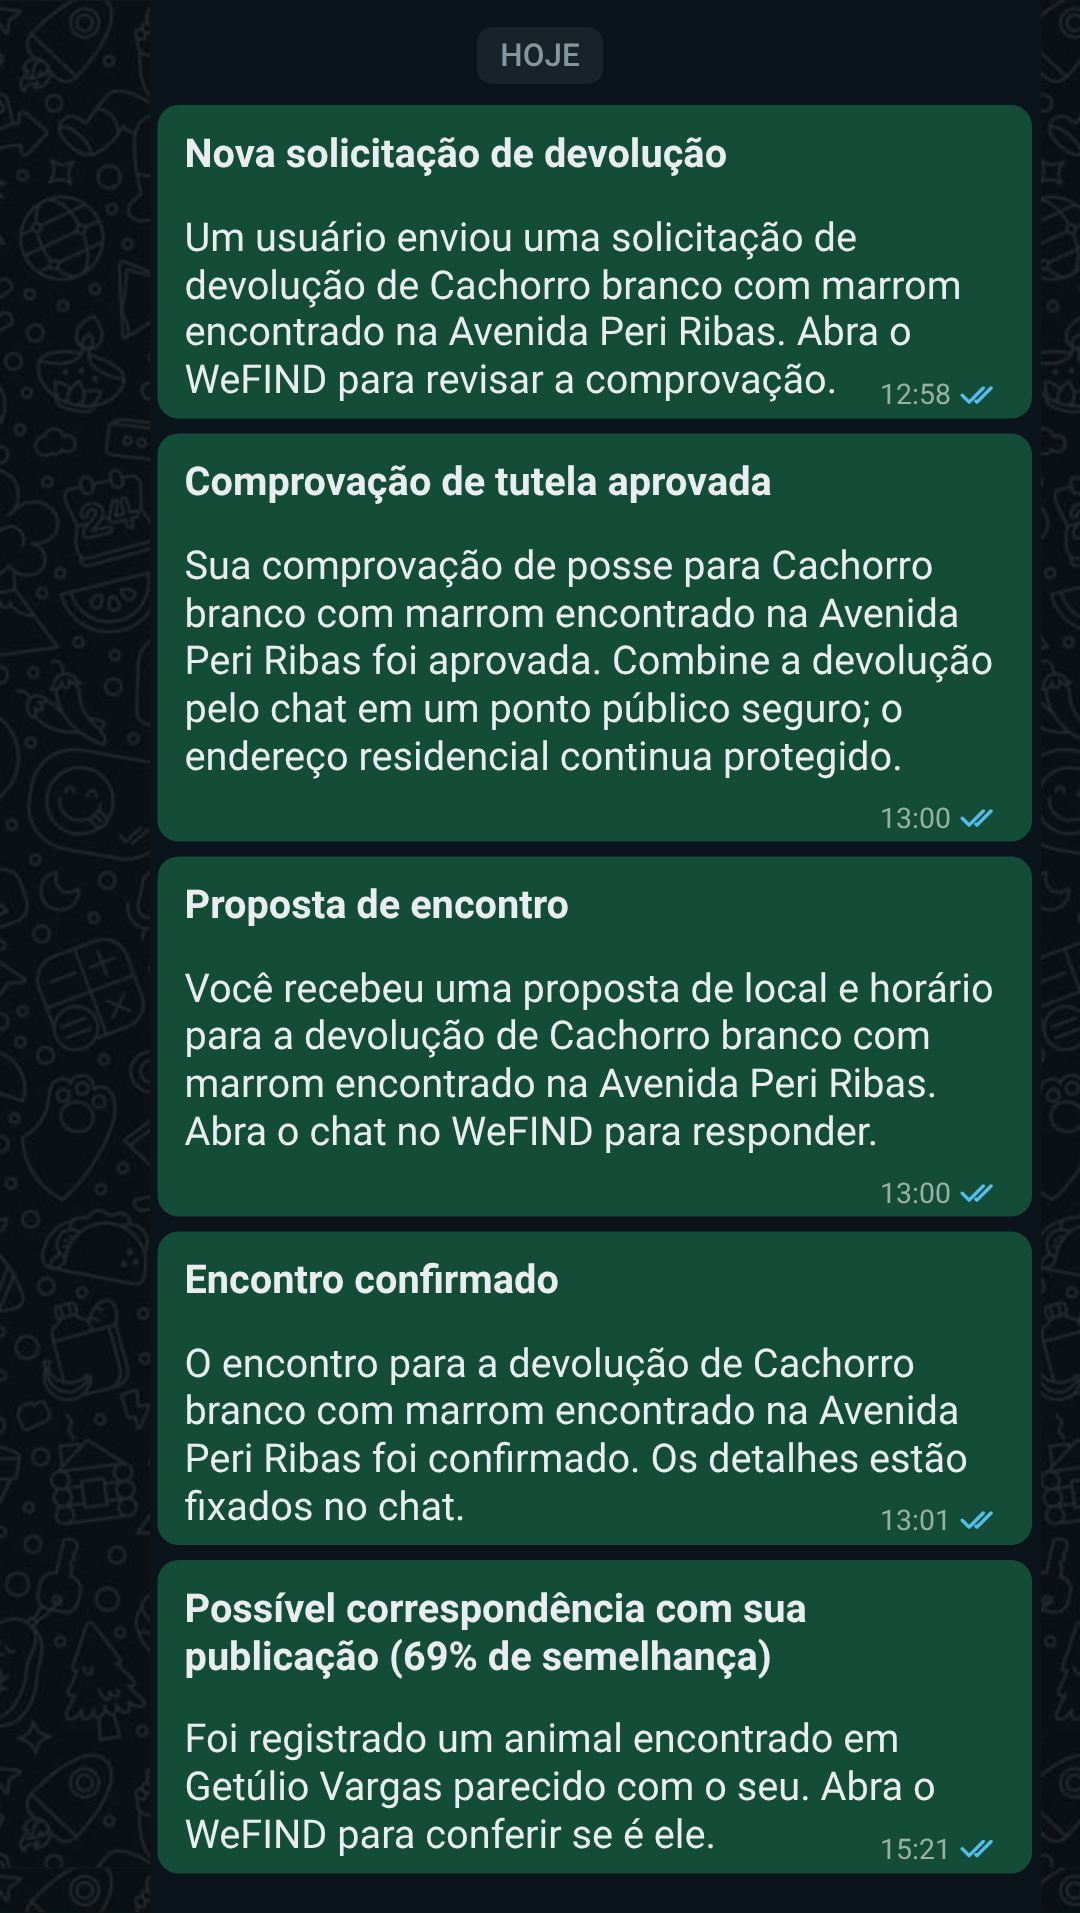
\includegraphics[width=0.5\textwidth]{imagens/04_telas_aplicativo/tela-notificacoes-whatsapp.png}
    \fonte{Autoria própria (2026)}
\end{figure}

No protótipo, as mensagens são enviadas pela Evolution API a partir do número de WhatsApp do próprio autor, conectado ao serviço para os testes. Por isso, no aparelho do autor, elas aparecem como enviadas por ele mesmo. Em uma versão em produção, o envio seria feito por um número institucional do WeFIND, e os códigos de verificação, que seguem pelo mesmo canal, não foram incluídos na figura.

A comprovação de tutela, descrita na Seção~\ref{sec:tutela}, começa na ficha de um animal encontrado e termina no chat, com o encontro de devolução combinado. A Figura~\ref{fig:tela_comprovacao_tutela} mostra a parte feita pelo tutor.

\begin{figure}[H]
    \centering
    \caption{Solicitação de Devolução pelo Tutor}
    \label{fig:tela_comprovacao_tutela}
    \vspace{0.15cm}
    \begin{minipage}[t]{0.31\textwidth}
        \centering
        \capturaTela{imagens/04_telas_aplicativo/tela-tutela-solicitar.jpeg}
        \par\vspace{0.12cm}
        {\small Figura~\thefigure.a) Ficha com Endereço Protegido}
    \end{minipage}
    \hfill
    \begin{minipage}[t]{0.31\textwidth}
        \centering
        \capturaTela{imagens/04_telas_aplicativo/tela-tutela-formulario.jpeg}
        \par\vspace{0.12cm}
        {\small Figura~\thefigure.b) Envio da Comprovação}
    \end{minipage}
    \hfill
    \begin{minipage}[t]{0.31\textwidth}
        \centering
        \capturaTela{imagens/04_telas_aplicativo/tela-tutela-em-analise.jpeg}
        \par\vspace{0.12cm}
        {\small Figura~\thefigure.c) Comprovação em Análise}
    \end{minipage}
    \par\vspace{0.12cm}
    \fonte{Autoria própria (2026)}
\end{figure}

Na Figura~\ref{fig:tela_comprovacao_tutela}.a, a ficha do animal acolhido mostra apenas a região do bairro e o aviso de endereço protegido, com o botão ``Solicitar devolução''. Na Figura~\ref{fig:tela_comprovacao_tutela}.b, o tutor escolhe como deseja comprovar a tutela (fotos do animal, carteira de vacinação ou marcas ocultas), anexa as imagens pela galeria ou pela câmera e escreve uma mensagem para quem acolheu o animal. Depois do envio, a ficha passa a exibir a comprovação como ``em análise'', com o endereço ainda protegido (Figura~\ref{fig:tela_comprovacao_tutela}.c), e uma mensagem automática abre a conversa com o autor da publicação.

Ao abrir essa conversa, quem está com o animal vê no alto a faixa ``Confirmar tutor e combinar encontro'', com o botão ``Liberar local''. Apesar do nome, esse botão não revela o endereço: se as fotos e as marcas conferem com o animal, ele o usa para propor um ponto de encontro público. A Figura~\ref{fig:tela_encontro_devolucao} mostra essa etapa.

\begin{figure}[H]
    \centering
    \caption{Combinação do Encontro de Devolução pelo Chat}
    \label{fig:tela_encontro_devolucao}
    \vspace{0.15cm}
    \begin{minipage}[t]{0.31\textwidth}
        \centering
        \capturaTela{imagens/04_telas_aplicativo/tela-tutela-proposta.jpeg}
        \par\vspace{0.12cm}
        {\small Figura~\thefigure.a) Proposta de Encontro}
    \end{minipage}
    \hfill
    \begin{minipage}[t]{0.31\textwidth}
        \centering
        \capturaTela{imagens/04_telas_aplicativo/tela-tutela-proposta-recebida.jpeg}
        \par\vspace{0.12cm}
        {\small Figura~\thefigure.b) Proposta Recebida pelo Tutor}
    \end{minipage}
    \hfill
    \begin{minipage}[t]{0.31\textwidth}
        \centering
        \capturaTela{imagens/04_telas_aplicativo/tela-tutela-encontro-confirmado.jpeg}
        \par\vspace{0.12cm}
        {\small Figura~\thefigure.c) Encontro Confirmado}
    \end{minipage}
    \par\vspace{0.12cm}
    \fonte{Autoria própria (2026)}
\end{figure}

Na Figura~\ref{fig:tela_encontro_devolucao}.a, quem acolheu o animal escolhe o ponto de encontro no mapa, o dia, o horário e, se quiser, uma observação, como a roupa que vai usar; o próprio formulário recomenda um local público e movimentado, como uma praça, um \textit{pet shop} ou uma clínica veterinária. Ao enviar a proposta, a comprovação é aprovada. O tutor recebe a proposta fixada no alto da conversa (Figura~\ref{fig:tela_encontro_devolucao}.b), com as opções ``Confirmar'', ``Outro horário'' e ``Não posso''. Depois da confirmação, o cartão muda para ``Encontro confirmado'' (Figura~\ref{fig:tela_encontro_devolucao}.c), com atalho para abrir o ponto no Google Maps e os botões para remarcar ou cancelar. Cada proposta e cada resposta também ficam registradas como mensagens na conversa.

Os animais oferecidos para adoção aparecem no mesmo mural das demais publicações, identificados pela etiqueta ``Para Adoção'', como mostra a Figura~\ref{fig:tela_adocao}. A ficha do animal segue o mesmo modelo das outras publicações, e o contato com quem o oferece acontece pelo chat.

\begin{figure}[H]
    \centering
    \caption{Publicação para Adoção no Mural}
    \label{fig:tela_adocao}
    \capturaTela{imagens/04_telas_aplicativo/tela-feed-adocao.jpeg}
    \fonte{Autoria própria (2026)}
\end{figure}

O perfil reúne as áreas pessoais do usuário, e cada membro também tem um perfil público, que outras pessoas podem consultar. A Figura~\ref{fig:tela_perfil} apresenta as duas telas.

\begin{figure}[H]
    \centering
    \caption{Perfil do Usuário e Perfil Público do Membro}
    \label{fig:tela_perfil}
    \vspace{0.15cm}
    \begin{minipage}[t]{0.48\textwidth}
        \centering
        \capturaTela{imagens/04_telas_aplicativo/tela-perfil-v2.jpeg}
        \par\vspace{0.12cm}
        {\small Figura~\thefigure.a) Perfil do Usuário}
    \end{minipage}
    \hfill
    \begin{minipage}[t]{0.48\textwidth}
        \centering
        \capturaTela{imagens/04_telas_aplicativo/tela-perfil-membro-v2.jpeg}
        \par\vspace{0.12cm}
        {\small Figura~\thefigure.b) Perfil Público}
    \end{minipage}
    \par\vspace{0.12cm}
    \fonte{Autoria própria (2026)}
\end{figure}

Na Figura~\ref{fig:tela_perfil}.a, o perfil do usuário dá acesso a Meus pets e carteirinhas, aos próprios anúncios, às solicitações de devolução, às configurações e à ajuda. A Figura~\ref{fig:tela_perfil}.b mostra o perfil público de um membro, com o número de publicações e de reencontros, a média das classificações recebidas, que aparece como ``Sem classificações'' enquanto ninguém avaliou o membro, e a atividade na comunidade, como avistamentos compartilhados e animais procurados; a aba ``Classificações'' reúne as avaliações recebidas, descritas na Seção~\ref{sec:classificacao}, e o perfil público não exibe e-mail nem telefone.

A área ``Meus pets'', descrita na Seção~\ref{sec:meus_pets}, é acessada pelo perfil do usuário. A Figura~\ref{fig:tela_meus_pets} apresenta a lista de animais cadastrados, o formulário de cadastro e a carteirinha digital.

\begin{figure}[H]
    \centering
    \caption{Meus Pets e Carteirinha Digital}
    \label{fig:tela_meus_pets}
    \vspace{0.15cm}
    \begin{minipage}[t]{0.31\textwidth}
        \centering
        \capturaTela{imagens/04_telas_aplicativo/tela-meus-pets.jpeg}
        \par\vspace{0.12cm}
        {\small Figura~\thefigure.a) Lista de Pets}
    \end{minipage}
    \hfill
    \begin{minipage}[t]{0.31\textwidth}
        \centering
        \capturaTela{imagens/04_telas_aplicativo/tela-cadastrar-pet.jpeg}
        \par\vspace{0.12cm}
        {\small Figura~\thefigure.b) Cadastro do Pet}
    \end{minipage}
    \hfill
    \begin{minipage}[t]{0.31\textwidth}
        \centering
        \capturaTela{imagens/04_telas_aplicativo/tela-carteirinha.jpeg}
        \par\vspace{0.12cm}
        {\small Figura~\thefigure.c) Carteirinha Digital}
    \end{minipage}
    \par\vspace{0.12cm}
    \fonte{Autoria própria (2026)}
\end{figure}

Na Figura~\ref{fig:tela_meus_pets}.a, cada animal cadastrado aparece com foto, características e número de microchip, acompanhado dos botões para ver a carteirinha, editar o cadastro e acionar o alerta ``Meu pet fugiu''. O formulário da Figura~\ref{fig:tela_meus_pets}.b reaproveita os mesmos seletores de espécie, sexo, porte, cor e faixa etária usados no cadastro de publicações, o que mantém os dados compatíveis com a busca por correspondências. A carteirinha da Figura~\ref{fig:tela_meus_pets}.c reúne a identificação do animal, o tutor, o contato de emergência, as indicações de castração e vacinação e um código QR, e pode ser salva ou compartilhada.

